% Generated by Sphinx.
\documentclass[a4paper,10pt]{manual}
\usepackage[utf8]{inputenc}
\usepackage[T1]{fontenc}
\title{Epigrass Documentation}
\date{July 07, 2008}
\release{2.0a1}
\author{Flavio Codeco Coelho}
\newcommand{\sphinxlogo}{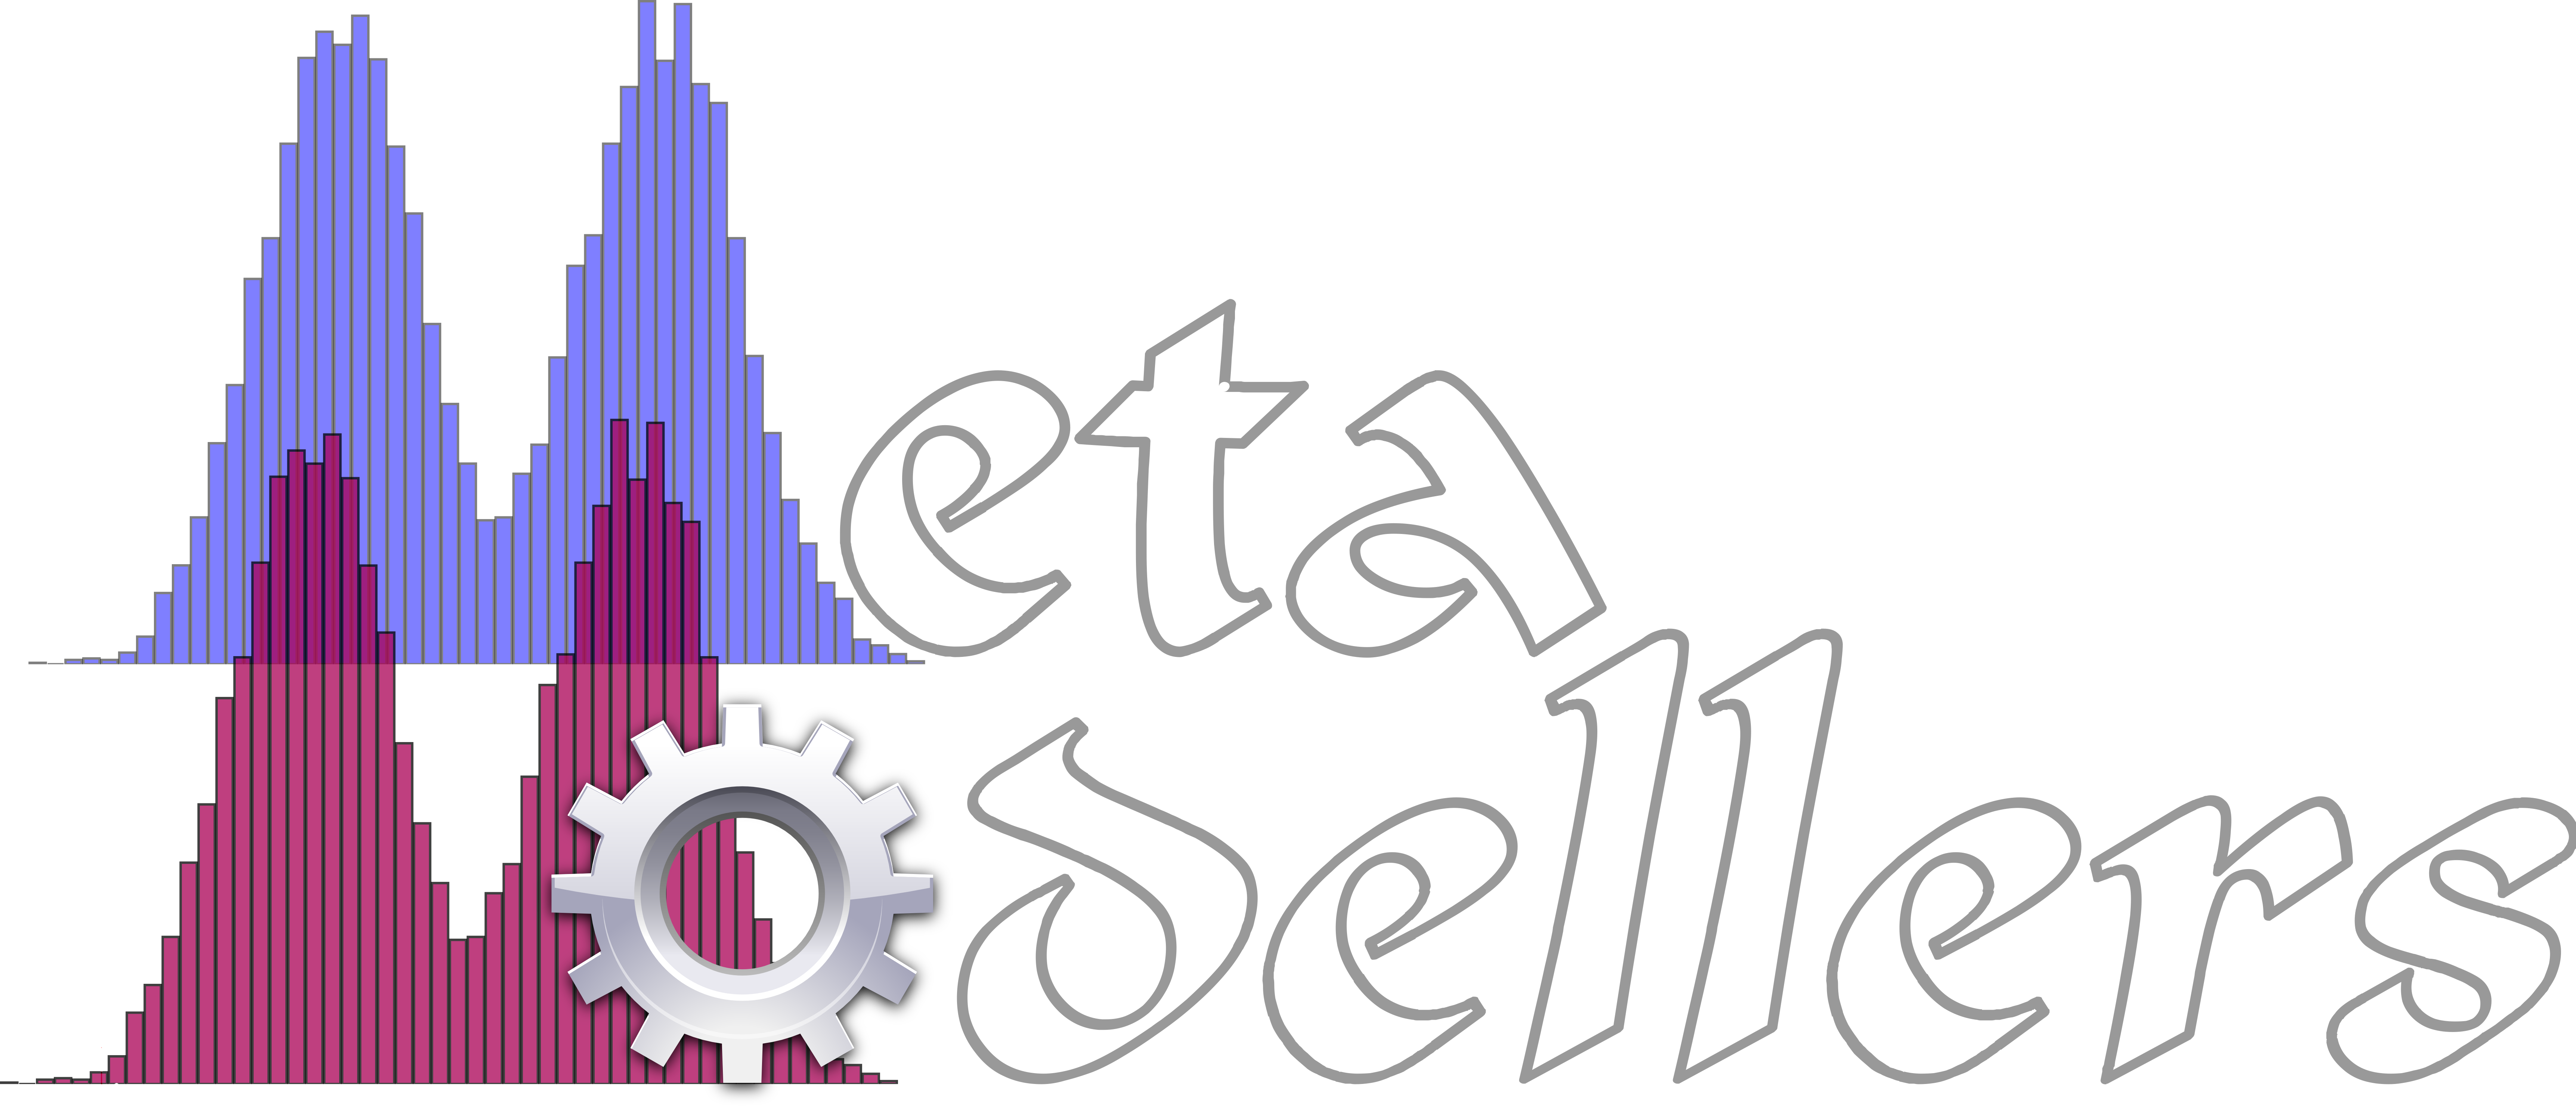
\includegraphics{MEMO_logo.png}\par}

\makeindex
\makemodindex
\newcommand\at{@}
\newcommand\lb{[}
\newcommand\rb{]}
\newcommand\PYGaz[1]{\textcolor[rgb]{0.00,0.63,0.00}{#1}}
\newcommand\PYGax[1]{\textcolor[rgb]{0.84,0.33,0.22}{\textbf{#1}}}
\newcommand\PYGay[1]{\textcolor[rgb]{0.00,0.44,0.13}{\textbf{#1}}}
\newcommand\PYGar[1]{\textcolor[rgb]{0.73,0.38,0.84}{#1}}
\newcommand\PYGas[1]{\textcolor[rgb]{0.25,0.44,0.63}{\textit{#1}}}
\newcommand\PYGap[1]{\textcolor[rgb]{0.78,0.36,0.04}{#1}}
\newcommand\PYGaq[1]{\textcolor[rgb]{0.38,0.68,0.84}{#1}}
\newcommand\PYGav[1]{\textcolor[rgb]{0.00,0.44,0.13}{\textbf{#1}}}
\newcommand\PYGaw[1]{\textcolor[rgb]{0.13,0.50,0.31}{#1}}
\newcommand\PYGat[1]{\textcolor[rgb]{0.32,0.47,0.09}{#1}}
\newcommand\PYGau[1]{\textcolor[rgb]{0.13,0.50,0.31}{#1}}
\newcommand\PYGaj[1]{\textcolor[rgb]{0.00,0.44,0.13}{#1}}
\newcommand\PYGak[1]{\textcolor[rgb]{0.14,0.33,0.53}{#1}}
\newcommand\PYGah[1]{\textcolor[rgb]{0.00,0.13,0.44}{\textbf{#1}}}
\newcommand\PYGai[1]{\textcolor[rgb]{0.73,0.38,0.84}{#1}}
\newcommand\PYGan[1]{\textcolor[rgb]{0.00,0.44,0.13}{\textbf{#1}}}
\newcommand\PYGao[1]{\textcolor[rgb]{0.25,0.44,0.63}{\textbf{#1}}}
\newcommand\PYGal[1]{\colorbox[rgb]{1.00,0.94,0.94}{\textcolor[rgb]{0.25,0.50,0.56}{#1}}}
\newcommand\PYGam[1]{\textbf{#1}}
\newcommand\PYGab[1]{\textit{#1}}
\newcommand\PYGac[1]{\textcolor[rgb]{0.25,0.44,0.63}{#1}}
\newcommand\PYGaa[1]{\textcolor[rgb]{0.19,0.19,0.19}{#1}}
\newcommand\PYGaf[1]{\textcolor[rgb]{0.25,0.50,0.56}{\textit{#1}}}
\newcommand\PYGag[1]{\textcolor[rgb]{0.13,0.50,0.31}{#1}}
\newcommand\PYGad[1]{\textcolor[rgb]{0.25,0.44,0.63}{#1}}
\newcommand\PYGae[1]{\textcolor[rgb]{0.13,0.50,0.31}{#1}}
\newcommand\PYGaZ[1]{\textcolor[rgb]{0.02,0.16,0.45}{\textbf{#1}}}
\newcommand\PYGbf[1]{\textcolor[rgb]{0.44,0.63,0.82}{\textit{#1}}}
\newcommand\PYGaX[1]{\textcolor[rgb]{0.00,0.44,0.13}{#1}}
\newcommand\PYGaY[1]{\textcolor[rgb]{0.25,0.44,0.63}{#1}}
\newcommand\PYGbc[1]{\textcolor[rgb]{0.00,0.44,0.13}{\textbf{#1}}}
\newcommand\PYGbb[1]{\textcolor[rgb]{0.13,0.50,0.31}{#1}}
\newcommand\PYGba[1]{\textcolor[rgb]{0.00,0.00,0.50}{\textbf{#1}}}
\newcommand\PYGaR[1]{\textcolor[rgb]{0.73,0.38,0.84}{#1}}
\newcommand\PYGaS[1]{\textcolor[rgb]{0.25,0.50,0.56}{\textit{#1}}}
\newcommand\PYGaP[1]{\textcolor[rgb]{0.25,0.44,0.63}{#1}}
\newcommand\PYGaQ[1]{\textcolor[rgb]{0.13,0.50,0.31}{#1}}
\newcommand\PYGaV[1]{\textcolor[rgb]{0.05,0.52,0.71}{\textbf{#1}}}
\newcommand\PYGaW[1]{\textcolor[rgb]{0.25,0.44,0.63}{#1}}
\newcommand\PYGaT[1]{\textcolor[rgb]{0.50,0.00,0.50}{\textbf{#1}}}
\newcommand\PYGaU[1]{\textcolor[rgb]{0.00,0.44,0.13}{#1}}
\newcommand\PYGaJ[1]{\textcolor[rgb]{0.25,0.44,0.63}{#1}}
\newcommand\PYGaK[1]{\textcolor[rgb]{0.02,0.16,0.49}{#1}}
\newcommand\PYGaH[1]{\fcolorbox[rgb]{1.00,0.00,0.00}{1,1,1}{#1}}
\newcommand\PYGaI[1]{\textcolor[rgb]{0.56,0.13,0.00}{#1}}
\newcommand\PYGaN[1]{\textcolor[rgb]{0.05,0.52,0.71}{\textbf{#1}}}
\newcommand\PYGaO[1]{\textcolor[rgb]{0.78,0.36,0.04}{\textbf{#1}}}
\newcommand\PYGaL[1]{\textcolor[rgb]{0.73,0.73,0.73}{#1}}
\newcommand\PYGaM[1]{\textcolor[rgb]{0.00,0.44,0.13}{#1}}
\newcommand\PYGaB[1]{\textcolor[rgb]{0.00,0.25,0.82}{#1}}
\newcommand\PYGaC[1]{\textcolor[rgb]{0.33,0.33,0.33}{\textbf{#1}}}
\newcommand\PYGaA[1]{\textcolor[rgb]{0.00,0.44,0.13}{#1}}
\newcommand\PYGaF[1]{\textcolor[rgb]{1.00,0.00,0.00}{#1}}
\newcommand\PYGaG[1]{\textcolor[rgb]{0.73,0.38,0.84}{#1}}
\newcommand\PYGaD[1]{\textcolor[rgb]{0.25,0.50,0.56}{\textit{#1}}}
\newcommand\PYGaE[1]{\textcolor[rgb]{0.63,0.00,0.00}{#1}}
\newcommand\PYGbg[1]{\textcolor[rgb]{0.00,0.44,0.13}{\textbf{#1}}}
\newcommand\PYGbe[1]{\textcolor[rgb]{0.40,0.40,0.40}{#1}}
\newcommand\PYGbd[1]{\textcolor[rgb]{0.25,0.44,0.63}{#1}}

\begin{document}
\maketitle
\tableofcontents



Contents:

\resetcurrentobjects


\chapter{Overview of Epigrass}

Epigrass is a platform for network epidemiological simulation and analysis. It enables researchers to perform comprehensive spatio-temporal simulations incorporating epidemiological data and models for disease transmission and control in order to create sophisticated scenario analyses.


\section{Components}

The Epigrass system is composed of 4 components, The Epigrass simulator, the Epigrass database, Epigrass visualization module, and the report generator. They can all be used separately but should be invoked through Epigrass' user interface.


\section{Modeling Approach}

The geographical networks  over which epidemiological processes take place can be very straightforwardly represented in a object-oriented framework. In such a framework, the nodes and edges of the geographical networks are objects with their attributes and methods.

Once the archetypal node and edge objects are defined with appropriate attributes and methods, then a code representation of the real system can be constructed, where cities (or other geographical localities) and transportation routes are instances of the node and edge objects, respectively. The whole network is also an object with a whole collection of attributes and methods.

This framework leads to a compact and hierarchical computational modelconsisting of a network object containing a variable number of node and edge objects. This framework also do not pose limitations to encapsulation, potentially allowing for networks within networks if desirable (not yet implemented).

For the end user this framework is transparent since it mimics the natural structure of the real system. Even after the model is converted into a code object all of its component objects remain accessible to the user.


\section{Geographical Network Models}
\index{shapefile}
Epigrass's geo-referenced models are built from two basic sources of data: a map (in shapefile format) which provide the cartographical base over which the models are represented and specific data about nodes and edges that are provided by the user for the network of interest.


\subsection{Defining the Cartographic Background}

If the user has a map for the georeferred data, this can be passed to Epigrass. In this case, the cartographic background is defined by defining the name of the shapefile file (with path relative to the working directory) in the model'.epg file. Along with the path to the shapefile,  the variable in the shapefile, which contains the geocode of localities and their name must also be specified:

\begin{Verbatim}[commandchars=@\[\]]
shapefile @PYGbe[=]  @lb[]@PYGad[']@PYGad[riozonas_LatLong.shp]@PYGad['],@PYGad[']@PYGad[nome_zonas]@PYGad['],@PYGad[']@PYGad[zona_trafe]@PYGad[']@rb[]
\end{Verbatim}

If the user does not have a map in shapefile format, he can still use Epigrass. In this case, the georeferred data is read only from two .csv files (more on that ahead).


\subsection{Defining Nodes}

A graph has nodes and edges. Nodes can be cities or other localities depending on the model being constructed. The definition of nodes require the setting of many attributes listed below. The nodes will have many more attributes defined at run-time which will depend on other aspects of the model, these will be discussed later.

The data necessary at build time to create nodes come from a CSV (comma-separated-values) ASCII-text file, with the following attributes, (in this order):
\begin{description}
\item[\emph{Latitude, Longitude}]
This attribute will be used to geo reference the  node. The coordinate system must match those used in the cartographic base imported from GRASS. Coordinates can be coded in either decimal or sexagesimal format.

\item[\emph{Name}]
Used for identification purposes only. It can be a city name, for instance.

\item[\emph{Population}]
Since the simulation models will all be of a populational nature. Population size must be specified at build time.

\item[\emph{Geocode}]
A Unique Geocode (a number) is required. It will be used as a label/index to facilitate  reference to specific nodes.

\end{description}


\subsection{Defining Edges}

In Epigrass' graphs, edges represent transportation routes. Similarly to nodes, edges are defined at build-time with a reduced set of attributes which will be extended at run-time. Epigrass also expects to get these attributes from a CSV file:
\begin{description}
\item[\emph{Source}]
The name of the source node. The edges are bi-directional, but the nodes are labeled source and destination for reference purposes.

\item[\emph{Destination}]
The name of the destination node.

\item[\emph{Forward migration}]
Migration rate from source to destination, in number of persons per unit of time.

\item[\emph{Backward migration}]
Migration rate from destination to source, in number of persons per unit of time.

\item[\emph{Length}]
Distance in kilometers (or another unit) from source to destination via the particular route (not straight line distance).

\item[\emph{Source's geocode}]
This is the unique numerical identifier used in the sites file.

\item[\emph{Destination's geocode}]
This is the unique numerical identifier used in the sites file.

\end{description}


\subsection{Defining models}

The word model in Epigrass can mean two distinct objects: The network model and the node's epidemic model.

Node objects, in an Epigrass model, contain well-mixed population dynamic models within them. These models determine the dynamics of epidemics within the particular environments of each node. Epigrass comes with a few standard epidemiological modelsindex\{Models!epidemiological models\} to choose from when setting up your network. Currently, The same model type is applied to every node although their parameterization is node-specific. Besides the built-in model types, users can define their own, as shown on chapter ref\{ch:usingepg\}.

Network modelsindex\{Models!network model\} are specified in a ASCII-text script file (see appendix ref\{script\}). Epigrass comes with a few demo Network models for the user to play with until he/she is confident enough to build their own. Even then, it is advisable to use the demo scripts provided as templates to minimize syntax errors.

The script on the appendix ref\{script\} specifies a network model with an stochastic SEIR (see ref\{cap:modeling\}) epidemic model in its nodes. The user should study this model and play with its parameters to understand the features of Epigrass. A step-by-step tutorial on how to edit the model script can be found on chapter ref\{ch:usingepg\}.


\section{The Simulation}

A simulation run in Epigrass consists of a series of tasks performed at each time step \footnotemark[1] .
\begin{description}
\item[\emph{Calculate migration}]
For all edges in the network, the number of persons traveling each way is determined for the current time-step.

\item[\emph{Run epidemic models}]
For each node in the network the epidemic demographics are updated based on the local number of infected and susceptible individuals which have been updated by the transportation system.

\end{description}

All aspects of the simulation such as number of passengers traveling on each edge, number of infected/susceptible on each node and etc., are recorded in a step-by-step basis. This complete record allows for the model to be analyzed after the simulation has been completed without having to recalculate it.


\subsection{Output}

The output of a simulation in Epigrass is three-fold: A graphical display which the animated outcome of the simulation,  a written report, and a database table with numeric results.


\subsubsection{Graphical display}

During a simulation, selected epidemiological variables are animated in a 3-dimensional rendering over the map of the region containing the network.


\subsubsection{Report Generation}

The report contains a detailed analysis of the network model and the simulations ran with it. The report generates a LaTeX source file and compiles it to a PDF document for visualization.

Three types of report are currently available:
\begin{description}
\item[\textbf{Report = 1}]
Returns a set of descriptors of the network, described in chapter

\item[\textbf{Report = 2}]
Returns a set of basic epidemiological measures and plots of the time series.

\item[\textbf{Report = 3}]
Report 1 + Report 2

\end{description}

Report Generation is an optional, though recommended, step done at the end of the simulation. For the report, descriptive statistics are generated for the network. These have to do with network topology and properties. Additional sections can be added to the report with basic statistical analyses of the output of pre-selected nodes \footnotemark[2] .


\subsubsection{Database output}
\index{Database!results table}\index{Database!epigrass database}
Time series of \textbf{L}, \textbf{S}, \textbf{E}, and \textbf{I}, from simulations, are stored in a MySQL database named \emph{epigrass} . The results of each individual simulation is stored in a different table named after the model's script name, the date and time the simulation has been run. For instance, suppose you run a simulation of a model stored in a file named \code{script.epg}, then at the end of the simulation, a new table in the epigrass database will be created with the following name: \emph{script\_Wed\_Jan\_26\_154411\_2005}. Thus, the results of multiple runs from the same model get stored independently.
\footnotetext[1]{
The number of time steps is defined in the model script
}\footnotetext[2]{
Listed in the siteRep variable at the script
}
\resetcurrentobjects


\hypertarget{install}{}\chapter{Building and Installing}

This chapter will walk through all aspects of Epigrass installation. From obtaining, building and installing  the prerequisites to the installation of Epigrass itself.

Most of the steps will be quite simple and similar since they will make use of standard tools for package installation on Debian GNU/Linux and derivatives. If you use a different distribution, you should check its documentation for package installation instructions.

If, on your distribution, a package is not available for the required version, you can try to obtain an updated version of the package at the web-sites provided. On the rare cases where pre-built packages are not available, instructions on how to build the software from source should also be available from its web-site.


\section{Required Packages}


\subsection{Python}
\begin{description}
\item[\emph{Web-site:}]
\href{http://www.python.org}{http://www.python.org}

\item[\emph{Version required:}]
\textgreater{}=2.5

\end{description}

Python is a simple yet powerful object-oriented language. Its simplicity makes it easy to learn, but its power means that large and complex applications can also be created easily. Its interpreted nature means that Python programmers are very productive because there is no edit/compile/link/run development cycle.

Python is probably installed automatically by your GNU/Linux distribution (it is on Debian). If not, it is best to use your distribution's standard tools for package installation. On Debian for example:

\begin{Verbatim}[commandchars=@\[\]]
@PYGai[$ ]sudo apt-get install python python-dev
\end{Verbatim}


\subsection{Numeric Python}
\begin{description}
\item[\emph{Web-site:}]
\href{http://www.scipy.org/numpy}{http://www.scipy.org/numpy}

\item[\emph{Version required:}]
\textgreater{}= 1.0

\end{description}

Numeric Python is a module for fast numeric computations in Python.

Example installation:

\begin{Verbatim}[commandchars=@\[\]]
@PYGai[$ ]sudo apt-get install python-numpy
\end{Verbatim}


\subsection{Matplotlib}
\begin{description}
\item[\emph{Web-site:}]
\href{http://matplotlib.sourceforge.net}{http://matplotlib.sourceforge.net}

\item[\emph{Version required:}]
\textgreater{}0.9

\end{description}

Matplotlib is a Module that provides plotting capabilities to Python.

\begin{Verbatim}[commandchars=@\[\]]
@PYGai[$ ]sudo apt-get install python-matplotlib python-matplotlib-data python-matplotlib-doc
\end{Verbatim}


\subsection{PyQt}
\begin{description}
\item[\emph{Web-site:}]
\href{http://www.riverbankcomputing.co.uk/pyqt}{http://www.riverbankcomputing.co.uk/pyqt}

\item[\emph{Version required:}]
\textgreater{}4.0

\end{description}

PyQt is a set of Python bindings for the Qt toolkit. PyQt combines all the advantages of Qt and Python. A programmer has all the power of Qt, but is able to exploit it with the simplicity of Python.

PyQt depends on the Qt libraries to run. This dependency will be taken care by the package installation tools of most distributions, which will automatically install the required version of Qt.

Example installation:

\begin{Verbatim}[commandchars=@\[\]]
@PYGai[$ ]sudo apt-get install python-qt4
\end{Verbatim}


\subsection{PyQwt}
\begin{description}
\item[\emph{Web-site:}]
\href{http://pyqwt.sourceforge.net/}{http://pyqwt.sourceforge.net/}

\item[\emph{Version required:}]
\textgreater{}5.0

\end{description}

PyQwt is a Python binding for the Qwt5 technical widget library. It is necessary for some os Epigrass' visualizations capabilities.

Example installation:

\begin{Verbatim}[commandchars=@\[\]]
@PYGai[$ ]sudo apt-get install python-qwt5-qt4
\end{Verbatim}


\subsection{MySQL}
\begin{description}
\item[\emph{Web-site:}]
\href{http://www.mysql.com}{http://www.mysql.com}

\item[\emph{Version required:}]
\textgreater{}5.0

\end{description}

MySQL is a fast, multi-threaded, multi-user SQL database server. If you have a MySQL server available in your LAN, you may skip this step after making sure you have permission to access and use it to store your data.

Example installation:

\begin{Verbatim}[commandchars=@\[\]]
@PYGai[$ ]sudo apt-get install mysql-server mysql-client python-mysqldb
\end{Verbatim}


\subsubsection{Post-install configuration}

After installing MySQL, you will need to create a new database in the server, called \emph{epigrass} and a user with all priviledges to access and modify it. This is the user Epigrass will use to interact with MySQL.


\subsection{R}
\begin{description}
\item[\emph{Web-site:}]
\href{http://www.r-project.org}{http://www.r-project.org}

\item[\emph{Version required:}]
The most recent.

\end{description}

\textbf{R} is a statistical computing platform whis is very useful to analyze the output of Epirass's models. The Epigrass source distribution includes some example \textbf{R} scripts to interact with Epigrass-generated data.

Example installations:

\begin{Verbatim}[commandchars=@\[\]]
@PYGai[$ ]apt-get install r-base
\end{Verbatim}

After installing R, start an interactive session, and install a few extra packages.

\begin{Verbatim}[commandchars=@\[\]]
@PYGai[$ ]R
> update.packages@PYGbe[()]
> install.packages@PYGbe[(]@PYGbd['RMySQL']@PYGbe[)]
> install.packages@PYGbe[(]@PYGbd['DBI']@PYGbe[)]
> install.packages@PYGbe[(]@PYGbd['lattice']@PYGbe[)]
\end{Verbatim}

section\{Installing Epigrass\}
If you got through all the steps above, it will be an easy task to install Epigrass. There is a \emph{.deb} package for installing Epirass on Debian and Ubuntu. However, since it is not maitained by the developers of Epigrass, It may very well be outdated.  So please download Epigrass's source tarball (something named \code{Epigrass\_someversion.tar.gz}) from Sourceforge and, after unpacking it to some temporary directory, install it by typing:

\begin{Verbatim}[commandchars=@\[\]]
@PYGai[$ ]sudo python setup.py install
\end{Verbatim}

If the installation proceeds without errors, you will have three new executables available on your system:
\begin{description}
\item[\emph{epigrass}]
This starts Epigrass graphical user interface (GUI).

\item[\emph{epirunner}]
This is a command line version of Epigrass. With it you can run models without invoking the GUI. It's great for batch simulations and for remote use. for a quick help, try ``epirunner -h''.

\item[\emph{epgeditor}]
A graphical editor of .epg models. A easy way to edit already existing models. Contains detailed explanations of every section of the EPG file. {\color{red}\bfseries{}:math:`x\_3+y`}

Unknown interpreted text role ``math''.


\end{description}

\resetcurrentobjects

\resetcurrentobjects

\resetcurrentobjects

\resetcurrentobjects


\chapter{Indices and tables}
\begin{itemize}
\item {} 
\emph{Index}

\item {} 
\emph{Module Index}

\item {} 
\emph{Search Page}

\end{itemize}
\renewcommand{\indexname}{Module Index}\printmodindex\renewcommand{\indexname}{Index}

\printindex
\end{document}
